\section{Revised Figure Evidence and Coordinate Semantics}\label{sec:revision_figures}
\subsection{Hourly Storms teaser: selected window and eligibility sweep}\label{sec:s_hourly_teaser}
Main-paper Figure~1 uses the separate December 1999 hourly pressure-anomaly experiment, not the 118-frame half-day evaluation. The saved full-month R20 overview contains 744 original hours. Its orange box selects frames 30--46 (2 December, 06:00--22:00 UTC; 17 profiles) and normalized output positions $[0.10,0.42]$. The selected original scalar columns are identical to the corresponding R5 columns. Source snapshots are frames 33, 34, 35, 37 and 42 (09:00, 10:00, 11:00, 13:00 and 18:00). They show supplied-grid anomalies with the same centered 192-hour baseline; marker coordinates belong to the retained $49\times49$, 250-km-smoothed analysis. The full-month direction and canvas remain fixed throughout the sweep.

The local conditions use the retained construction. P preserves the hierarchy; R1, R2 and R5 use eligibility fractions $\kappa/\Delta_F=0.01$, $0.02$ and $0.05$, respectively. This fraction restricts merge relaxations and does not bound the measured output error. Each condition is solved forward from the original frame 0 through frame 96, retaining its own incoming temporal history; the selected window is not reset or assigned a newly fitted direction. The recomputed R20 prefix reproduces the saved full-month scalar columns exactly, with maximum anchor discrepancy $2.22\times10^{-16}L$. These additional illustrative layouts do not change the 614-frame or 325-input evaluation populations.

Letters $A,B,C,D,E,F$ identify computational tracks 7, 5, 8, 9, 10 and 0. At 09:00, $A$ is at $20.714^\circ$W, $31.586^\circ$N and $B$ at $15.000^\circ$W, $66.012^\circ$N. At 13:00, $A$ is at $22.143^\circ$W, $32.227^\circ$N and $C$ at $12.143^\circ$W, $66.012^\circ$N. At 18:00, $D$, $E$ and $F$ are at $(23.571^\circ\mathrm{W},32.874^\circ\mathrm{N})$, $(22.143^\circ\mathrm{W},53.085^\circ\mathrm{N})$ and $(12.143^\circ\mathrm{W},64.705^\circ\mathrm{N})$. Track 10 is the computed minimum associated with the Anatol context. Positive-overlap matching supplies these labels without independently verifying meteorological identity. $B$ ceases to be an independent tracked extremum after 09:00; $C$ receives a new identifier at 12:00. Geographic proximity does not establish a physical B--C identity. Only feature/hour pairs present in the five displayed snapshots receive markers; the scientific profiles retain all hourly values.

The directional-order examples are checked on saved references and anchors: R5 restores $A/B$ at 09:00, R1 restores $A/C$ at 13:00, and R2 restores $E/F$ at 18:00. The unchanged position of $A$ at 09:00 and 10:00 gives a separate layout-motion example: both references are $0.339258L$, but the P anchors are $0.237936L$ and $0.347592L$; R5 uses $0.347592L$ at both hours. Thus the illustrated jump is not a geographic displacement.

\begin{table}[H]\centering\small
\caption{Direct measurements for the 17-hour selected window, over all retained extrema and all leaf pairs in the full profiles. These values are illustrative window summaries, not additions to the main evaluation.}
\begin{tabular}{lrrr}\toprule
Condition & Mean position error (\%$L$) & Max position error (\%$L$) & Max merge error (hPa)\\\midrule
P & 2.3765 & 10.1323 & 0\\
R1 & 2.0710 & 10.1323 & 0.2580\\
R2 & 1.6700 & 10.1323 & 0.4260\\
R5 & 0.8996 & 2.5427 & 1.1549\\\bottomrule
\end{tabular}\label{tab:s_hourly_teaser}
\end{table}

All panels share the $[-35,35]$\,hPa display scale. Conservative anchor-aligned reconstruction preserves every original 4096-row hourly column, falling back to fixed-position interpolation across unsupported order changes or large jumps. Intermediate columns are display samples, not observations. Original coordinates, arrays, direct merge measurements, display checks and editable figure sources are frozen in \path{evidence/storms_teaser20261026/}.

\subsection{Source identities and selected frames}
The feature-linked figures read frozen arrays in \path{results/real_case_studies/evidence/}. No feature extraction, layout construction, persistence change, or experiment is rerun. Storms frame 48 is the previously retained witness. Wildfires frame 18 maximizes hierarchy cost among above-trigger frames with a persistent three-frame triple and positive position gain and scalar cost, with earliest ties. Tangaroa frame 140 maximizes achieved P-to-R displacement reduction among above-trigger frames with a persistent triple and positive scalar cost. These descriptive selection rules emphasize visible mechanisms; all performance summaries remain the complete-sequence results.

The underlying rows identify extrema by retained leaf IDs and positive-overlap track IDs. A track born within the enlarged window begins there; no trace is extrapolated to an absent feature. All scalar values, anchor coordinates, and error summaries come from saved records. Markers use the processed-field extrema over the raw source observations or pre-TTK volume views.

\begin{table}[H]\centering\small
\caption{Selected-frame evidence. Position quantities are percentages of fixed reference extent; NMLE is percentage of the processed sequence range. Tangaroa $H$ is a lower bound. These rows are separate cases, not a pooled mean.}
\begin{tabular}{lrrrrrr}\toprule
Case/frame & Leaves & Packing & $H$ & Max P & Max R20 & Actual NMLE\\\midrule
Storms/48 & 5 & 0 & 8.4484 & 8.8665 & 0.8333 & 13.2079\\
Wildfires/18 & 10 & 0 & 13.9211 & 14.7545 & 2.6328 & 15.0944\\
Tangaroa/140 & 27 & 0.1827 & $\ge13.7442$ & 14.7605 & 1.0164 & 13.7502\\\bottomrule\end{tabular}
\end{table}

\paragraph{Analytical cost and rendered measurement.} The planar event JSON fields named \path{actual_max_merge_error} were populated from the filling routine's returned analytical $\delta^*$, before the positive strict-extremum clearance. Direct all-pair checks on the saved complete columns give Storms frame 48: analytical 12.557166\,hPa, measured 12.558173\,hPa (13.207872\% NMLE); Wildfires frame 18: analytical 0.635061777, measured 0.635062968 (15.094425\% NMLE). The revised frame-level text and captions use the measurements. The original JSON and all 177 protected result files remain unchanged; the correction is documented in the revision checks. Sequence-level main tables already use the independently measured filling records.

\subsection{Coordinate transformations and display resolution}
A temporal panel covering frames $l,\ldots,r-1$ maps frame $t$ to $x=x_0+(t-l+1/2)w/(r-l)$. Its vertical mapping is $y=y_0+(b-v)h/(b-a)$ for the displayed ordinate range $[a,b]$. Complete maps use $[0,1]$; local windows explicitly label cropped ranges. TMTM and ST-MTM normalize their own native sample domains to this unit interval. Only RG maps identify that interval with the fixed directional reference. Dashed reference tracks appear only in RG panels.

The scalar images are nearest-neighbour displays of the frozen profiles. Tangaroa's cached 4096-row display may omit narrow extrema at nearby rows. Exact full-resolution anchors are therefore overlaid independently from the retained positions; they are not snapped to the preview colours. All Tangaroa metrics use the 131072-row outputs, not these previews.

Storms source layers use the existing geographic transformation and coastline, with each extremum transformed from its processed-grid position. Wildfires source layers retain the full $[0,120]^2$ domain, unsmoothed raw log-FRP observations, and the saved processed extrema. Main-paper Figure~9 uses a light yellow--orange--brown palette with unchanged linear normalization: processed maps use $[0,4.207268783]$ and raw snapshots use $[0,12.050886763]$. Artificial negative connection values use grey-blue. The five main-paper raw snapshots have equal domain scale, and track labels terminate at the last saved sample. The original three-frame comparison remains in S10. Additional source-view records are in \path{evidence/dimensional_results/source_views.json}. Palette and coordinate records are retained in \path{evidence/figure8_display/}. Three Tangaroa images come from \path{tangaroa_volumes.npz}, frames 139, 140, and 141. For the framed views in main-paper Figure~15, the same original-grid scalar frames are rendered with the original transfer function and an orthographic display camera yawed by $18^\circ$ from the preceding view. One affine projection maps the volume, all eight domain corners, and the marked three-dimensional extrema to the image plane. The display camera and projected coordinates are retained in \path{evidence/figure9_display/}; the original camera cache remains unchanged. Volume aspect and source-field aspect remain fixed. The accompanying editable markers remain separate from the scientific raster layers.

\begin{table}[H]\centering\small
\caption{Tangaroa frame-140 extrema and fixed-reference coordinates. Local feature IDs are original-grid vertex IDs.}
\setlength{\tabcolsep}{4pt}
\begin{tabular}{lrrrrrr}\toprule
Track & Leaf & $x$ & $y$ & $z$ & Reference & R anchor\\\midrule
A/432 & 361559 & $-0.152676$ & 0.118994 & $-0.489916$ & 0.290592 & 0.280428\\
B/462 & 981499 & 0.315552 & $-0.196089$ & $-0.469748$ & 0.803567 & 0.813727\\
C/388 & 2674152 & 0.492809 & 0.011732 & $-0.417647$ & 0.533667 & 0.543827\\\bottomrule\end{tabular}
\end{table}

\subsection{Exact frontier and selected-order aggregation}
Figure~5 averages exact per-frame frontiers under a common scalar budget: $\overline F(D)=T^{-1}\sum_tF_{T_t}(D)$. A selected-order working point uses $\overline\tau=T^{-1}\sum_t\tau(\pi_t)$ and $D_{\max}=\max_t\delta^*(\pi_t)$. Every selected order is feasible at $D_{\max}$, so $\overline F(D_{\max})\le\overline\tau$. The plotted vertical gap quantifies search/order choice at that common budget. It does not compare a mean scalar error to a maximum budget, and it does not replace measured anchor residuals. At R20 the Storms point is $(26.0704\%,1.5841\%L)$, whereas the common-budget attainable mean is $1.1068\%L$.

Figure~\ref{fig:s_certificate_fill}(c) keeps the selected R20 orders fixed and averages original-LCA versus optimal scalar costs: Storms 2.0711\% versus 1.4680\%, Wildfires 4.6789\% versus 3.9551\%, and Ring 5.4579\% versus 2.7289\%. Main-table NMLE is independently measured after filling and includes strict-extremum clearance. Figure~4 is the supplied three-leaf schematic: $A/B$ joins at $s_1$ and the outside leaf joins at $s_2$. For equal leaf values below their midpoint, order $A,C,B$ gives original-LCA cost $s_2-s_1$ and optimal cost $(s_2-s_1)/2$. The former saved five-leaf profiles remain separate numerical evidence (LCA cost 5, optimal cost 2.5); they are no longer the source of Figure~4.

\paragraph{Current frontier population.} Main-paper Figure~5 shows the five current planar temporal sequences, including 366 annual PM2.5 fields. The 611/614-frame frontier check uses the active datasets defined in the evaluation protocol. Historical Storms 2013/14 and January PM2.5 remain supplementary controls.

\begin{figure}[H]\centering
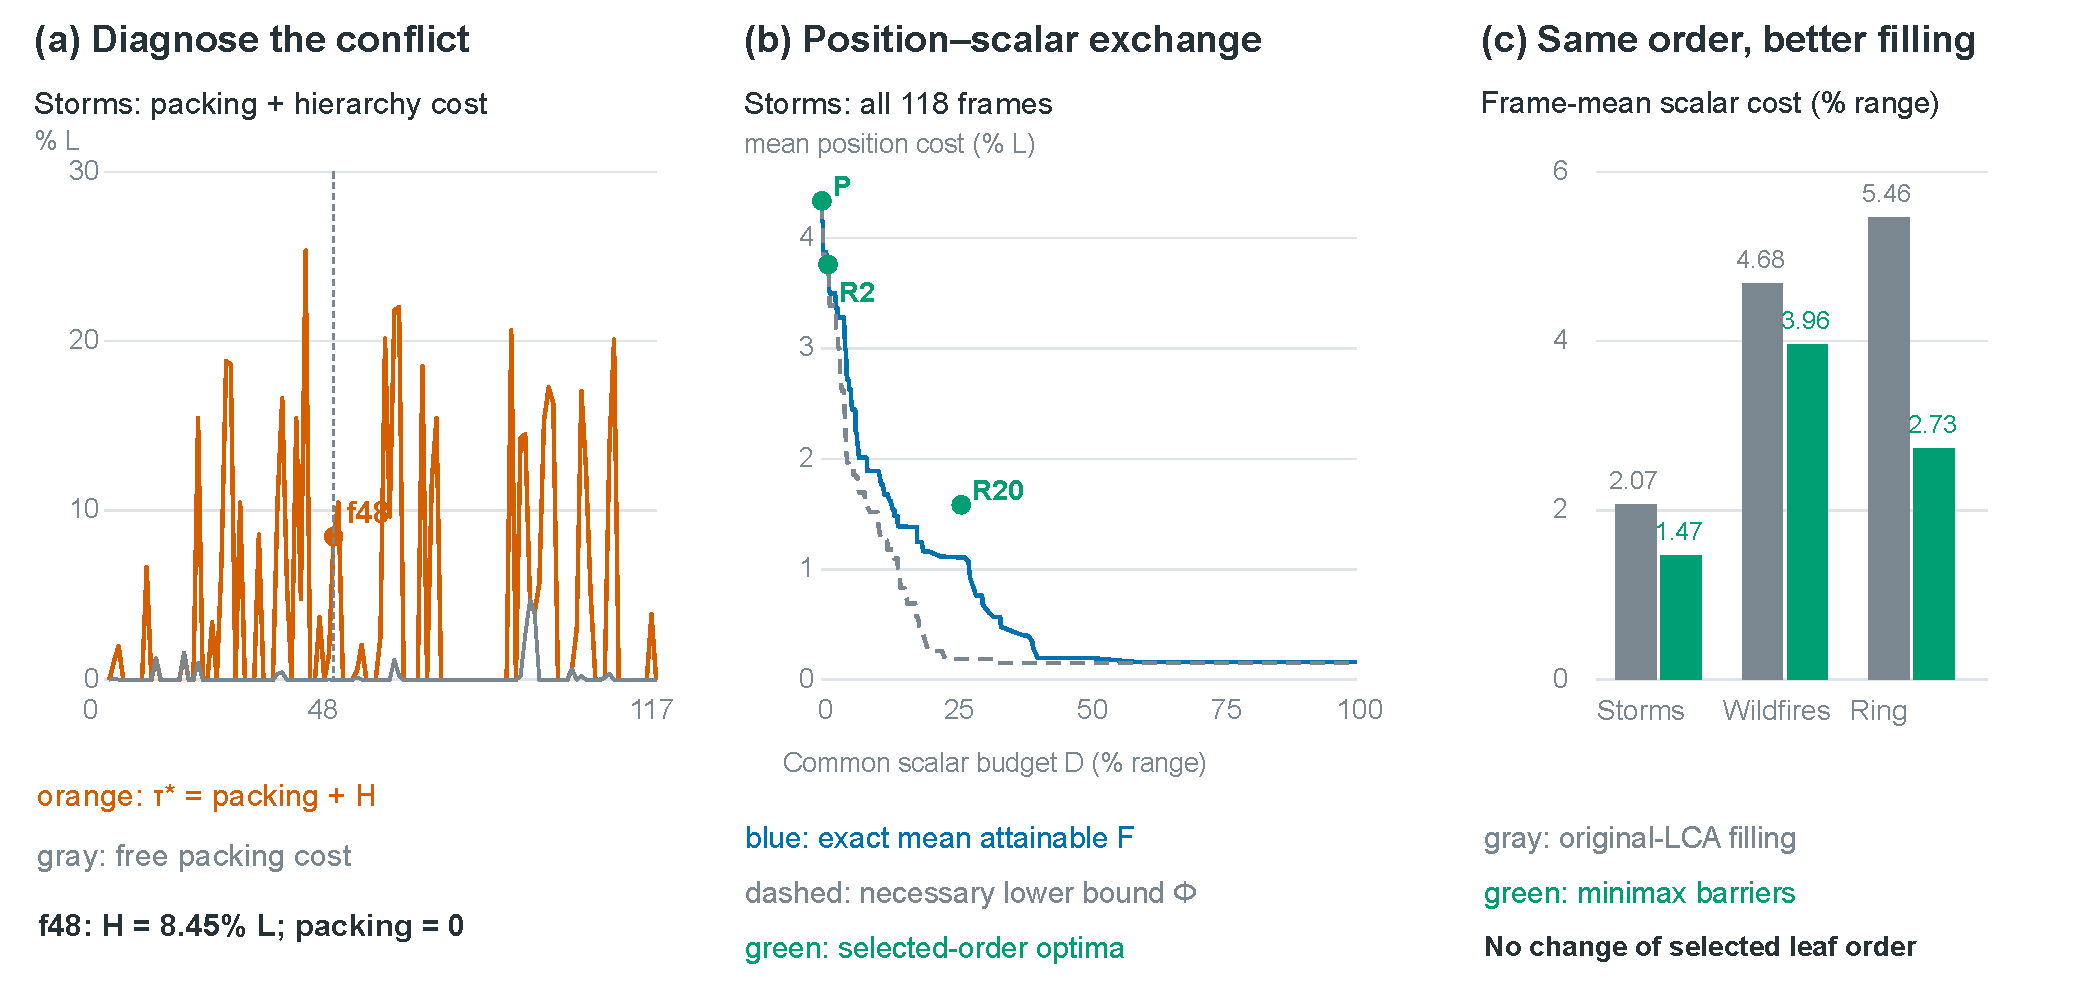
\includegraphics[width=\linewidth]{figures/Supplement_PositionScalarDiagnostic.pdf}
\caption{Additional certificate and filling diagnostics retained from the preceding revision. (a) Storms interval certificate, free packing cost, and the frame-48 hierarchy conflict. (b) Common-budget mean frontier and selected-order working points. (c) Mean original-LCA and optimal scalar costs for the same selected R20 orders. These supporting diagnostics accompany the five-panel main-paper frontier overview.}
\label{fig:s_certificate_fill}\end{figure}

\subsection{Storms three-snapshot detail}
The following retained four-method comparison complements Figure~1's separate hourly overview and eligibility-window comparison. It adds source snapshots at frames 47, 48, and 49 using identical colours and true extremum positions. Missing features are unmarked; $A=60$ begins at frame 48. Baseline axes remain native layout ranks, and dashed references occur only in RG panels.
\begingroup
\setlength{\intextsep}{6pt}
\begin{figure}[H]\centering
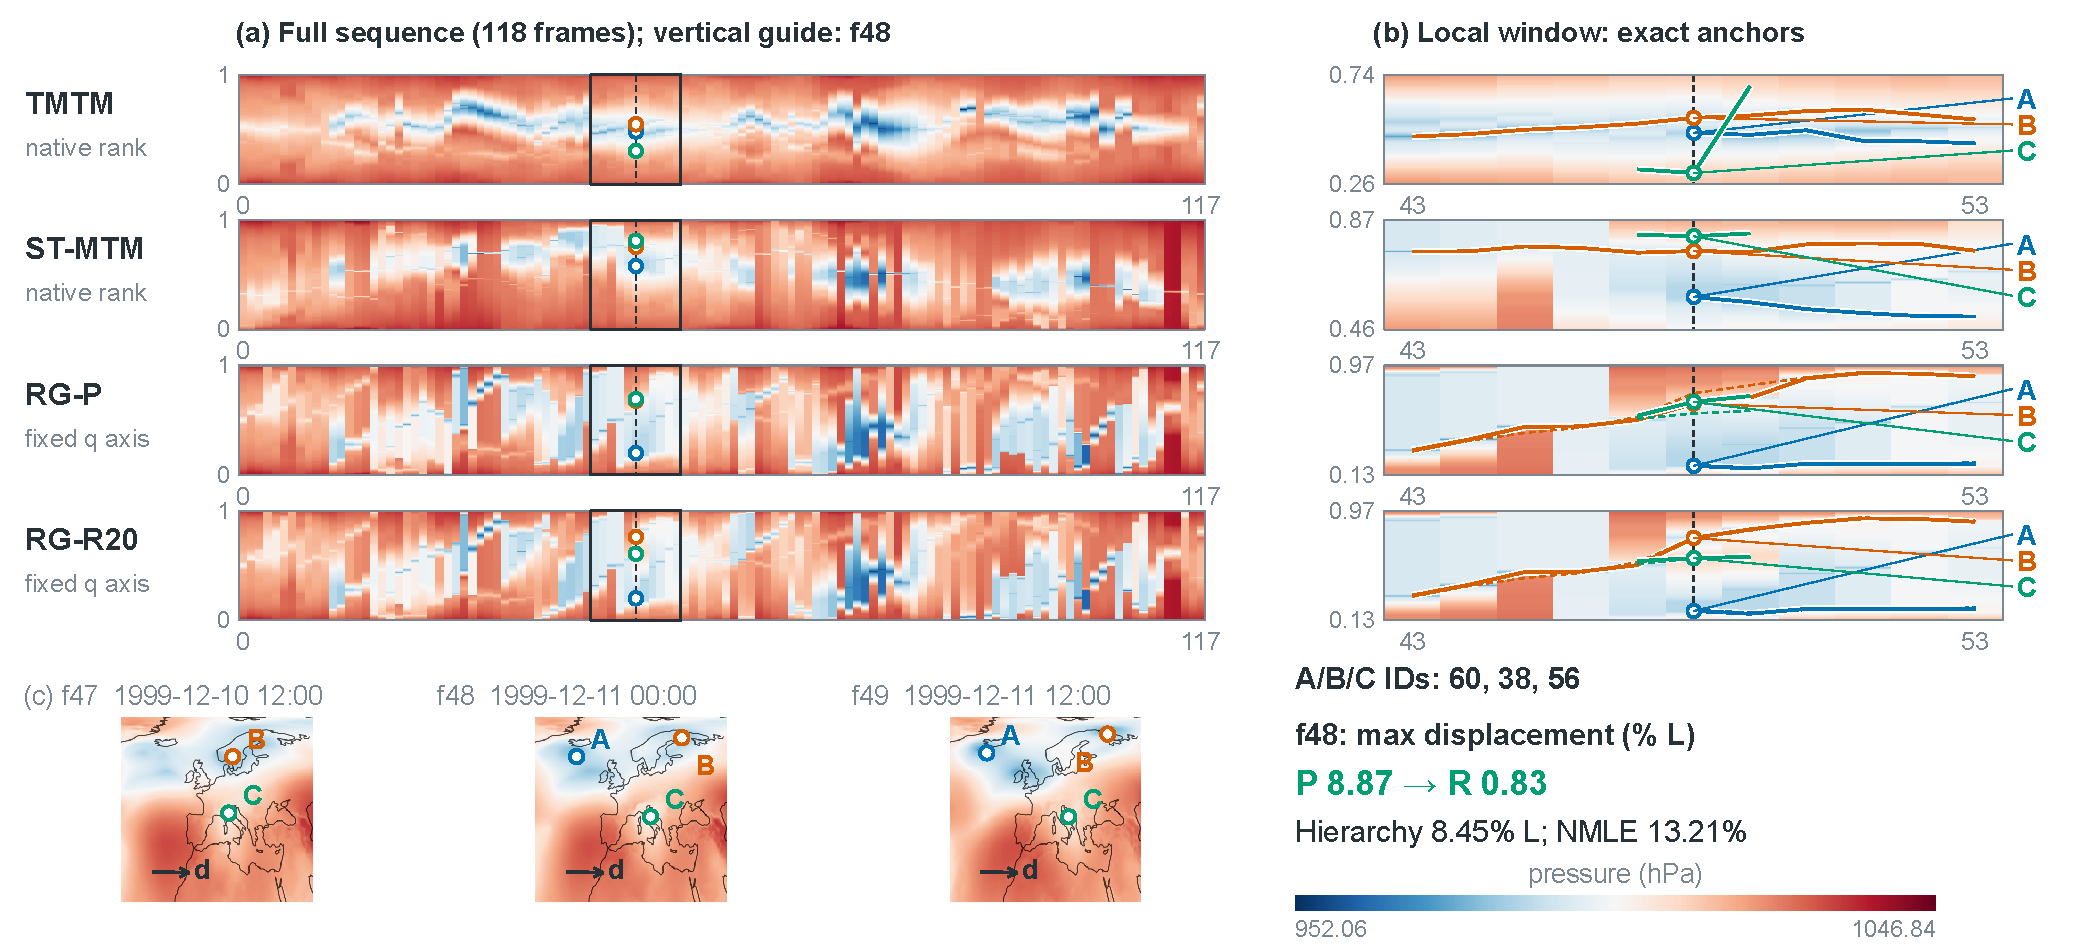
\includegraphics[width=.90\linewidth]{figures/Supplement_Storms_Detail.pdf}
\caption{Storms detail for the 118-frame quantitative sequence: four layouts, the local conflict window, and raw source snapshots with saved processed extrema. Tracks $A=60$, $B=38$, and $C=56$ refer to this sequence. Main-paper Figure~1 instead uses a separate 744-hour pressure-anomaly visualization with its own extracted features and track identifiers; the two populations and scalar preprocessing are distinct.}
\end{figure}
\endgroup

\paragraph{Storms eligibility and fixed-order scalar cost.} At frame 48, the $A/B$ node's parent gap is 15.314\,hPa and meets the eligibility threshold $\kappa=19.016$\,hPa. Its half-gap lower bound is 7.657\,hPa. Fixing $C$'s extremum value at 1006.693\,hPa raises the chosen order's analytical optimum to 12.557\,hPa; strict-extremum clearance produces the independently measured 12.558\,hPa error. These quantities respectively describe eligibility, a necessary bound, the fixed-order optimum, and the rendered result.


\subsection{Detailed measurements accompanying the Results section}
\paragraph{Storms frame 48.} Tracks $A=60,B=38,C=56$ have normalized references 0.208, 0.759, 0.603. TMTM orders them $C,A,B$, ST-MTM/P use $A,B,C$, and R20 uses $A,C,B$. All-leaf NROE is 19.734\%, 7.779\%, 7.779\%, and zero, respectively. Maximum P/R displacement is 8.867\%/0.833\% of $L$. Source merges are 994.136\,hPa for $A/B$ and 1009.449\,hPa for either outside pair; R places all three at 1006.694\,hPa.

\paragraph{Wildfires frames 17--19.} Track $C=52$ has fixed reference 0.418, P anchors 0.281, 0.549, 0.325, and R anchors 0.468, 0.422, 0.409. At frame 18, $A=3,B=48,C=52$ have references 0.169, 0.685, 0.418. Hierarchy cost is $13.921\%L$; maximum P/R displacement is $14.754\%/2.633\%L$. All-leaf NROE for TMTM/ST-MTM/P/R20 is 38.026\%/38.026\%/13.318\%/1.587\%. The $A/B$ source level 0.060800 changes to $-0.574262$, giving worst-pair error 0.635063 and 15.094\% actual NMLE.

\begin{samepage}
\paragraph{Tangaroa frame 140.} Tracks $A=432,B=462,C=388$ have references 0.291, 0.804, 0.534 and source joins 0.713403 ($A/B$), 0.869923 (either outside pair). TMTM/P/R20 order them $C,A,B$/$A,B,C$/$A,C,B$, with all-leaf NROE 15.529\%/13.495\%/0.532\%. Packing is $0.183\%L$, the hierarchy lower bound $13.744\%L$, and maximum P/R displacement $14.760\%/1.016\%L$. R sets $A/B$ to 0.988407 and $A/C$ to 0.594919: worst-pair change 0.275004, or 13.750\% actual NMLE.
\end{samepage}

\subsection{Annual PM2.5 source-linked case}
The current main-paper PM2.5 case is additional visual analysis of the existing 366-frame experiment; no date, grid, smoothing parameter, layout, match, or primary metric is replaced. Of 34 frames with a strongest three-feature witness exceeding $0.02L$, frames 185, 186, 195, 196, and 317 have the witness tracks present for at least three consecutive saved dates. Their median witness obstruction selects frame 195 (July 14), with bound $10.2575\%L$. The three tracks coexist on frames 195--197. The displayed window is frames 191--201 (July 10--20), including all saved births and deaths. Supplied views are frames 193--197; no temporal averaging or additional smoothing is introduced for those images. Each file represents its recorded 10:30 field, without an established daily averaging interval.

The July 14 measurements use displayed raster anchors, rather than the continuous-coordinate $E_\infty$ of the main sequence table. Exact source-array checks give maximum P/R20 errors $14.8809\%L$/$0.8373\%L$. Source/P pair levels are 25.936435 ($A/B$) and 22.626129 ($A/C,B/C$); R20 uses 24.281282 for all three. Direct labelled merge measurement yields 1.655153\,$\mu$g\,m$^{-3}$, normalized by the fixed annual processed range 147.885866\,$\mu$g\,m$^{-3}$, or 1.119210\% NMLE. The window maximum is 3.332004\%. Colour scales are shared within panels: 0--165 for the annual map and 0--100\,$\mu$g\,m$^{-3}$ for all local supplied/processed views and P/R20 maps. These display ranges do not redefine NMLE normalization. Province outlines are geographic context only.

The case selection, complete candidates, source hashes, marker coordinates, saved lifetimes, scalar comparisons, and display-reconstruction checks are packaged in \path{evidence/pm25_case20261023/}. The annual P/R20 primary motion errors remain 42/95 and 47/95. A local reference-alignment example is not a physical-event validation or an annual performance estimate.
